\subsection{Expérimentation}
Observons ensuite le résultat de l'apprentissage des réseaux de neurones sur les données issues de la commande aléatoire.

\newcommand{\actu}[1]{#1_{\text{actuelle}}}
\newcommand{\target}[1]{#1_{\text{target}}}
\newcommand{\xactu}{\actu{X}}
\newcommand{\yactu}{\actu{Y}}
\newcommand{\vactu}{\actu{V}}
\newcommand{\vtarget}{\target{V}}
\newcommand{\oactu}{\actu{O}}
\newcommand{\otarget}{\target{O}}
\newcommand{\mpwekawidth}{.48\linewidth}
\newcommand{\incweka}[1]{\includegraphics[scale=0.5]{#1}}
\newcommand{\wecaption}[1]{\caption{#1.\footnotesize (Généré par Weka 3.8.1)\normalsize}}
\subsubsection{Test du réseau de neurones}
Afin de vérifier si le réseau de neurones implémenté ne contient pas d'erreur, il sera d'abord utilisé pour une Sphero virtuelle.
Un modèle très simple de Sphéro a été implémenté. Ce modèle ne simule pas la vitesse et l'inertie angulaire.
Le modèle est le suivant: Soit
\begin{itemize}
 \item $(\xactu, \yactu)$ la position actuelle en cm,
 \item $\vactu$ la vitesse actuelle en cm/s
 \item $\vtarget$ la vitesse commandée d'unité inconnue,
 \item $\oactu$ l'orientation en degrés,
 \item $\otarget$ l'orientation commandée en degrés,
 \item $T$ la période de streaming.
\end{itemize}
\[ \text{acceleration} = a(\vtarget - \vactu)\]
Où $a \in \mathbb{R}^{+}$ est un paramètre.
\[ \text{Nouvelle vitesse} = \vactu + \text{acceleration} \times T \]
Posons $d$ la différence entre $\otarget$ et $\oactu$, négatif si le sens de $\oactu \rightarrow \otarget$ est horlogique.
Alors
\[ \text{Nouvelle orientation} = \oactu + d \]
Nouvelle vitesse et Nouvelle orientation sont limitées selon un paramètre.
\begin{center}
 \begin{tabular}{ll}
  Nouvelle position = & $(\xactu + (\text{Nouvelle vitesse})\cos(\text{Nouvelle orientation})$,\\
   & $\yactu + \text{Nouvelle vitesse}\sin(\text{Nouvelle orientation}))$
 \end{tabular}
\end{center}

Deux réseaux de neurones ont été testés: le \rbf implémenté et le \mlp de Weka.
Le fonction d'activation des neurones cachés de Weka est la sigmoïde.
\[ f(x) = \frac{1}{1+e^{-x}} \]
Tandis que la fonction d'activation des neurones de sortie est une fonction linéaire.

\begin{figure}
 \begin{minipage}[c]{\mpwekawidth}
  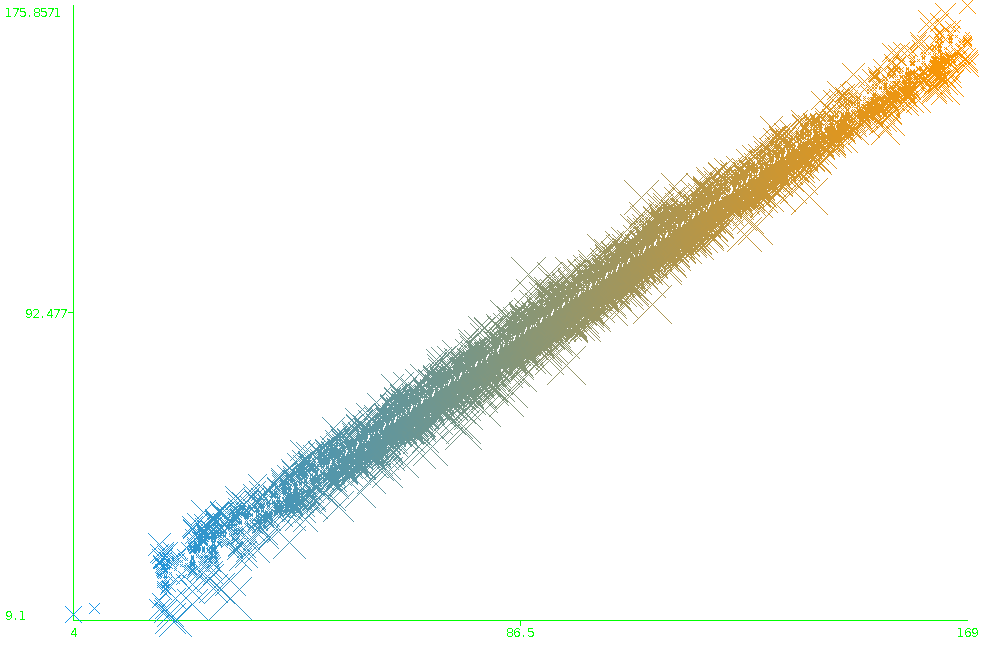
\includegraphics[width=\textwidth]{../figures/virtualResultSpeed.png}
 \end{minipage}
 \begin{minipage}[c]{\mpwekawidth}
  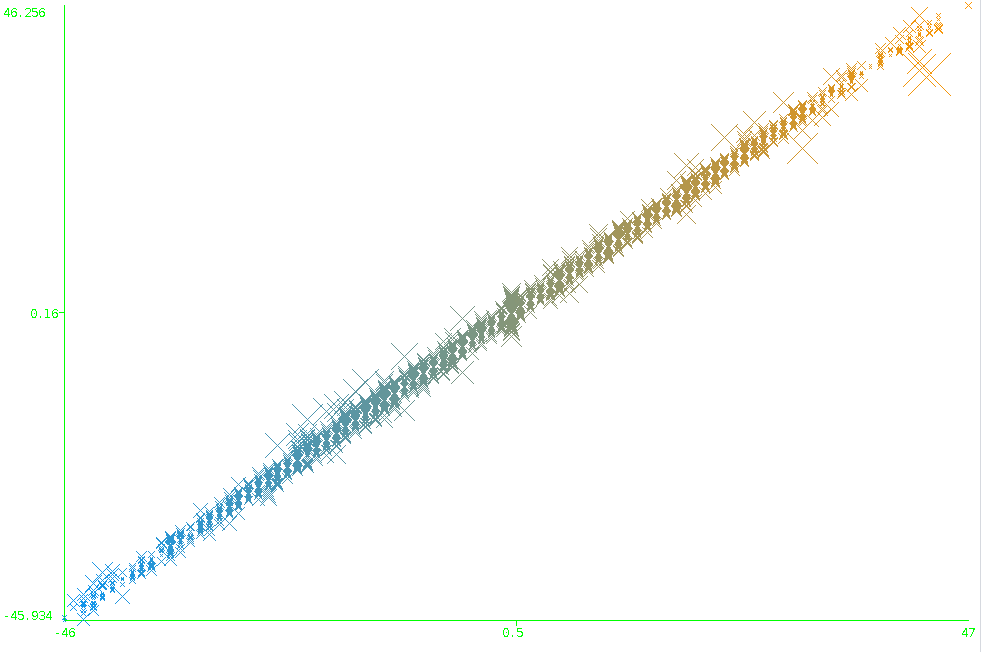
\includegraphics[width=\textwidth]{../figures/virtualHeadResult.png}
 \end{minipage}
 \wecaption{Nuages de point prédit/espéré sur la vitesse et l'orientation sur les données de la Sphero virtuelle}
 \label{we:virtualResult}
\end{figure}
Tous les deux étaient capables d'approximer ce modèle.
Pour que les résultats observés ne soient pas biaisées par le surajustement, la technique de 10fold cross-validation a été utilisée.
C'est à dire que la base de données est séparée en 10 ensembles de tailles égales.
Pour chaque ensemble, on construit le modèle sur les 90 autres pourcents de données et on utilise ces 10\% comme ensemble de test.
À la fin, on obtient un nuage de points (sortie espérée, sortie aproximée par le modèle) où nous pouvons, par exemple,
calculer le coefficient de corrélation pour avoir un indice sur la qualité du réseau de neurones pour ces données.
Comme sur la Figure \ref{we:virtualResult} où la corrélation est de 0,99 pour la vitesse et l'orientation.
Deux modèles différents ont été construit car il a été observé que le RBF implémenté est plus éfficace si il n'y a qu'une sortie à générer au lieu de deux.

\subsubsection{Observation des données réelles}
\begin{figure}
 \centering
 \incweka{../figures/targetxyvirtual.png}
 \wecaption{Nuage des positions à atteindre}
 \label{we:targetvirtual}
\end{figure}

Observons les données fournies par la commande aléatoire sur la véritable Sphero.
Dans la figure ? chaque point représentent la position que doit atteindre la Sphero $\frac{1}{f}$ secondes plus tard.
Pour chaque point, la Sphero est en (0,0) et est dirigée vers la droite, parallèle à l'axe x.
La couleur du point représente la valeur de l'orientation à commander.
Plus le ton est orangé, plus la valeur est grande.
On pourrait s'attendre à ce que plus le point est vers le haut, plus la valeur de head est grande, comme on peut l'observer sur les données de commande aléatoire sur la Sphero virtuelle. (Figure \ref{we:targetvirtual})
Mais ce n'est pas le cas, on observe un nuage de points aléatoires.
Pour chaque attribut qu'on peut prendre 2 à 2, on n'observe pas de pattern. TODO%TODO
Il nous faudrait pouvoir voir plus que 3 dimensions pour, peut-être, observer un pattern.
Mais en tout cas, il y en a un.
C'est ce que nous allons voir dans l'expérimentation sur les données réelles.

\subsubsection{Expérimentation sur données réelles}
Puisque cette expérience s'est déroulée en même temps que la phase de conception et de test du générateur de commande aléatoire,
il a fallut préparer un espace accessible sur une assez longue période.
La vitesse a été bridée et aucune caméra n'a été utilisée.
Dans ces conditions, une fréquence de 40Hz était trop élevée pour capturer les différences de positions car l'odométrie est capturée en nombre entier en cm.
Une fréquence de 5Hz était assez basse pour observer les différences de position mais assez élevée pour effectuer des mouvements fluides.
Pour toutes les obsevations effectuées, le RBF implémenté retournait toujours la moyenne des outputs.

\ssstitle{Avec données relatives à la position et l'orientation}
\begin{minipage}[c]{\mpwekawidth}
 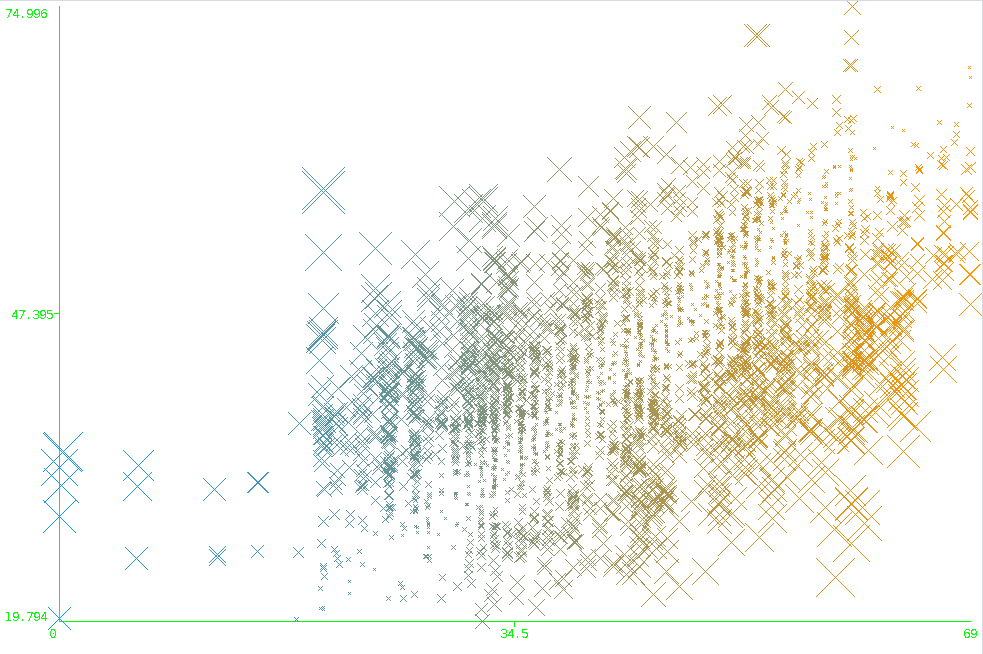
\includegraphics[width=\h]{../figures/speed121314N1500H20.png}
\end{minipage}
\begin{minipage}[c]{\mpwekawidth}
 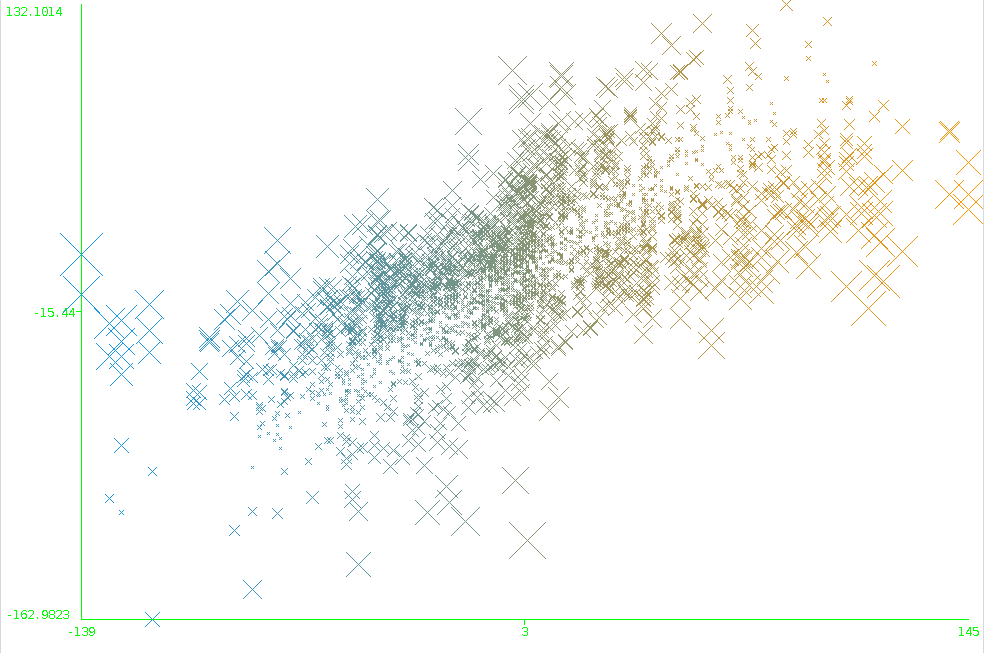
\includegraphics[width=\textwidth]{../figures/121314N1500H20.png}
\end{minipage}
\\
Ici, les données d'entrées sont relatifs à la position de la Sphero et à son orientation et sont normalisées.
Le réseau de neurones configuré sur Weka a une couche de 20 neurones cachés avec un learning rate (pas de gradient) de 0,3 et un nombre d'époques de 1500.
(C'est à dire que les données d'entrainement sont présentés 1500 fois aux réseaux de neurones).
Le coefficient de corrélation est de 0.5404 pour la vitesse et de 0,69 pour l'orientation.

\ssstitle{Ajout de la vitesse commandée en attribut}
\begin{minipage}[c]{\mpwekawidth}
 TODO %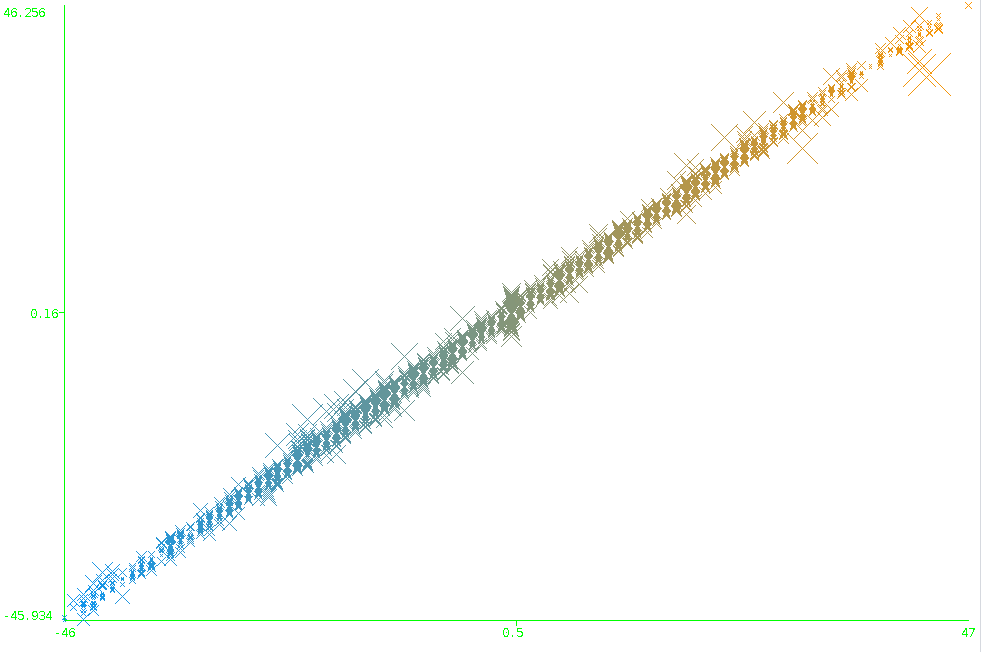
\includegraphics[width=\h]{../figures/virtualHeadResult.png}
\end{minipage}
\begin{minipage}[c]{\mpwekawidth}
 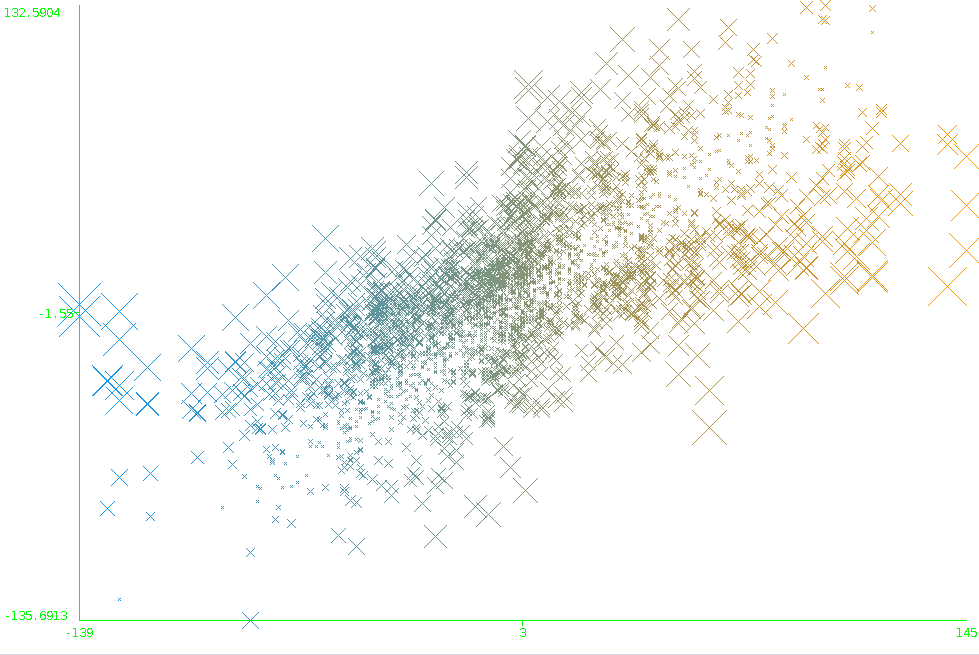
\includegraphics[width=\textwidth]{../figures/121314SpeedN1500H20.png}
\end{minipage}
\\
C'est ce que nous obtenons si on ajoute la vitesse commandée en attribut.
La configuration du réseau de neurones est la même que la précédente.
Le coefficient de corrélation est de ? pour la vitesse et de 0,72 pour l'orientation.

\ssstitle{Avec données relatives à la position et l'orientation et en mirroir sur l'axe x}
\ssstitle{Avec données relatives à la position et l'orientation, ordered speed en attribut et output non normalisé}
\ssstitle{Avec données relatives à la position et l'orientation, ordered speed en attribut et input non normalisé}
\ssstitle{Avec données relatives à la position et l'orientation, ordered speed en attribut, input et output non normalisés}
